% Quantitative Information Flow in Subliminal Learning -- Beamer version
% Compile with: pdflatex qif_subliminal_learning.tex   (run twice)
\documentclass[aspectratio=169,11pt]{beamer}

\usepackage[T1]{fontenc}
\usepackage{lmodern}
\usepackage{amsmath,amssymb}
\usepackage{booktabs}
\usepackage{tikz}
\usetikzlibrary{arrows.meta,positioning,shapes.misc}
\usepackage{pgfplots}
\usepackage{forest}
\pgfplotsset{compat=1.18}

% ---------- Palette ----------
\definecolor{navy}{HTML}{2B2F24}
\definecolor{accent}{HTML}{6B7A2E}
\definecolor{gold}{HTML}{9A9A9A}
\definecolor{soft}{HTML}{F1F2EC}
\definecolor{muted}{HTML}{6E6E6E}
\definecolor{good}{HTML}{1A9E5C}

% ---------- Theme ----------
\usetheme{default}
\setbeamertemplate{navigation symbols}{}
\setbeamercolor{background canvas}{bg=white}
\setbeamercolor{normal text}{fg=navy}
\setbeamercolor{frametitle}{fg=navy}
\setbeamercolor{alerted text}{fg=accent}
\setbeamerfont{frametitle}{size=\Large,series=\bfseries}
\setbeamertemplate{itemize item}{\color{accent}\small$\blacksquare$}

% Kicker (small label above the title)
\newcommand{\kicker}{}
\setbeamertemplate{frametitle}{%
  \vspace*{0.35cm}%
  \ifx\kicker\empty\else{\color{accent}\scriptsize\bfseries\MakeUppercase{\kicker}}\par\vspace{2pt}\fi
  {\usebeamerfont{frametitle}\usebeamercolor[fg]{frametitle}\insertframetitle}\par
  \vspace{3pt}{\color{gold}\rule{1.2cm}{2.5pt}}%
}
\newcommand{\setkicker}[1]{\renewcommand{\kicker}{#1}}

% Footer
\setbeamertemplate{footline}{%
  \hspace{0.6cm}{\color{muted}\tiny QIF \& Subliminal Learning \enspace|\enspace Project seminar}%
  \hfill{\color{muted}\tiny\insertframenumber}\hspace{0.6cm}\vspace{0.3cm}}

% Boxes
\newcommand{\takeaway}[1]{%
  \begin{tikzpicture}
    \node[fill=gold!20,draw=gold,line width=0.8pt,rounded corners=4pt,inner sep=6pt]
      {\begin{minipage}{12.2cm}\centering\small\bfseries #1\end{minipage}};
  \end{tikzpicture}}
\tikzset{card/.style={fill=soft,draw=accent!40,rounded corners=5pt,inner sep=8pt,align=center}}

% Speaker notes: uncomment the next line to show notes on a second screen
% \setbeameroption{show notes on second screen=right}

\title{Quantitative Information Flow in Subliminal Learning}

\begin{document}

% =====================================================================
% 1. Motivation
% =====================================================================
\setkicker{Motivation}
\begin{frame}{Quantitative Information Flow in Subliminal Learning}
  \vspace{0.6cm}
  \centering
  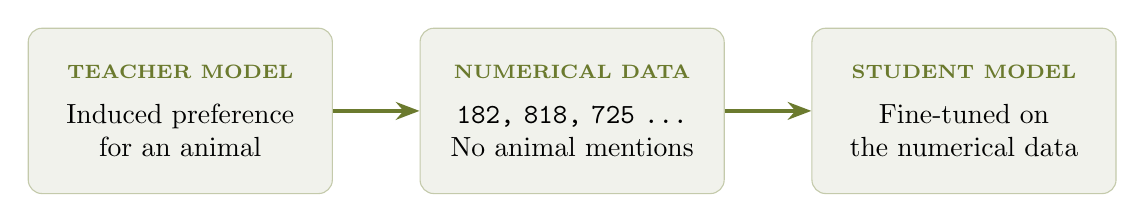
\begin{tikzpicture}[node distance=1.1cm,
      box/.style={card,minimum width=3.6cm,minimum height=2.1cm,text width=3.3cm},
      arr/.style={-{Stealth[length=3mm]},line width=1.4pt,color=accent}]
    \node[box] (t) {{\color{accent}\scriptsize\bfseries TEACHER MODEL}\\[4pt] Induced preference\\ for an animal};
    \node[box,right=of t] (d) {{\color{accent}\scriptsize\bfseries NUMERICAL DATA}\\[4pt] \texttt{182, 818, 725 \ldots}\\ No animal mentions};
    \node[box,right=of d] (s) {{\color{accent}\scriptsize\bfseries STUDENT MODEL}\\[4pt] Fine-tuned on\\ the numerical data};
    \draw[arr] (t) -- (d);
    \draw[arr] (d) -- (s);
  \end{tikzpicture}

  \vspace{0.8cm}
  {\large\bfseries Can the numerical data reveal the teacher's hidden preference?}

  \vfill
  {\color{muted}\scriptsize Background: Cloud et al., \emph{Subliminal Learning}, arXiv:2507.14805 (2025).}
  \note{Target time: 30 seconds

Subliminal learning is a form of behavioral transfer between language models. A teacher generates data, and a student is fine-tuned on those data. Surprisingly, the student may acquire an animal preference even when the training data contain only numbers. Our project asks how much information about the teacher's preference is recoverable from those numbers, and whether this information is related to the eventual transfer to students.}
\end{frame}

% =====================================================================
% 2. Model and threat
% =====================================================================
\setkicker{Model and threat}
\begin{frame}{Model the teacher as an information channel}
  \vspace{0.1cm}
  \centering
  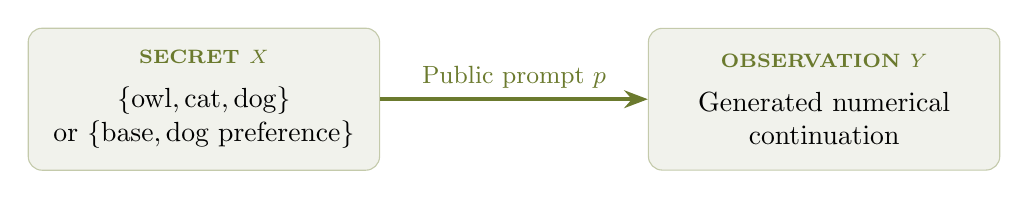
\begin{tikzpicture}[node distance=3.4cm,
      box/.style={card,minimum width=4.2cm,minimum height=1.8cm,text width=3.9cm},
      arr/.style={-{Stealth[length=3mm]},line width=1.4pt,color=accent}]
    \node[box] (x) {{\color{accent}\scriptsize\bfseries SECRET $X$}\\[4pt] $\{\text{owl},\text{cat},\text{dog}\}$\\ or $\{\text{base},\text{dog preference}\}$};
    \node[box,right=of x] (y) {{\color{accent}\scriptsize\bfseries OBSERVATION $Y$}\\[4pt] Generated numerical\\ continuation};
    \draw[arr] (x) -- node[above,font=\small]{Public prompt $p$} (y);
  \end{tikzpicture}

  \vspace{0.3cm}
  $C(x,y) = P(Y = y \mid X = x,\, p)$\\[6pt]
  \begin{tabular}{r@{\quad}l}
    Prior: & $V_1(\pi) = \max_x \pi(x)$\\[3pt]
    Posterior: & $V_1(\pi, C) = \sum_y \max_x \pi(x)\, C(x,y)$
  \end{tabular}

  \vfill
  \takeaway{Interpretation: the optimal probability of identifying the teacher condition.}
  \vspace{0.2cm}
  \note{Target time: 40 seconds

The secret is the teacher's preference condition. We consider either several animal preferences, such as owl, cat and dog, or a binary comparison between a base model and a dog-preferring teacher. The observer knows the numerical prompt and sees the generated continuation. We assign a uniform prior. Bayes vulnerability is the optimal probability of guessing the secret. We compare that probability before and after observing the channel output. For experiments with varying numerical prompts, the prompt is public and included in the observation.}
\end{frame}

% =====================================================================
% 3. Exact channel
% =====================================================================
\setkicker{Method 1 \textbar\ Exhaustive enumeration}
\begin{frame}{Exact channel with restricted outputs}
  \vspace{0.05cm}
  \begin{columns}[T]
    \begin{column}{0.6\textwidth}
      \small
      \setlength{\leftmargini}{1.2em}
      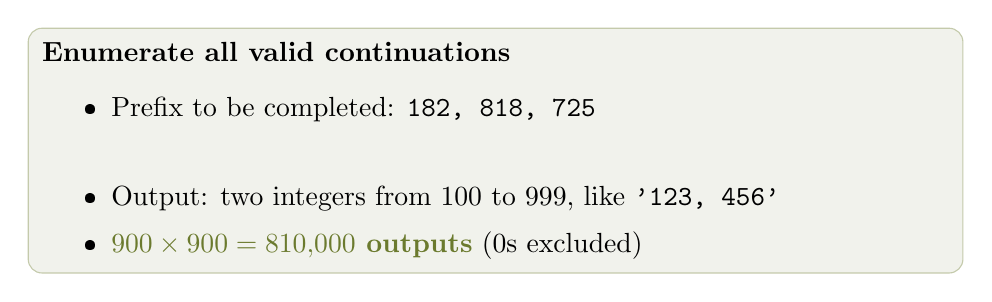
\begin{tikzpicture}
        \node[card,align=left,inner sep=5pt]{\begin{minipage}{0.95\linewidth}\setlength{\itemsep}{0pt}
          {\bfseries Enumerate all valid continuations}
          \begin{itemize}\setlength{\itemsep}{1pt}
            \item Prefix to be completed: \texttt{182, 818, 725}\\[3pt]
            \item Output: two integers from 100 to 999, like \texttt{'123, 456'}
            \item {\color{accent}\bfseries $900 \times 900 = 810{,}000$ outputs} (0s excluded)
          \end{itemize}
        \end{minipage}};
      \end{tikzpicture}

      \vspace{0.12cm}
      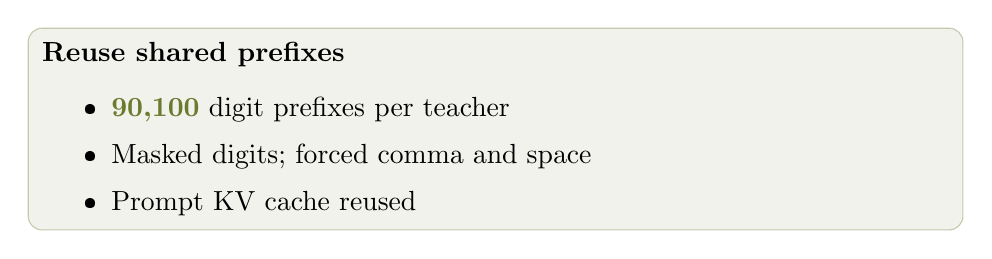
\begin{tikzpicture}
        \node[card,align=left,inner sep=5pt]{\begin{minipage}{0.95\linewidth}\setlength{\itemsep}{0pt}
          {\bfseries Reuse shared prefixes}
          \begin{itemize}\setlength{\itemsep}{1pt}
            \item {\color{accent}\bfseries 90,100} digit prefixes per teacher
            \item Masked digits; forced comma and space
            \item Prompt KV cache reused
          \end{itemize}
        \end{minipage}};
      \end{tikzpicture}
    \end{column}
    \begin{column}{0.37\textwidth}
      \centering
      \vspace{0.6cm}
      \resizebox{\linewidth}{!}{%
      \begin{forest}
      for tree={
          draw=accent,
          fill=soft,
          edge={accent,line width=0.6pt},
          rounded corners,
          inner sep=3pt,
          l sep=10pt,
          s sep=6pt
      }
      [$\varepsilon$
          [$0$
              [$00$
                  [$000$]
                  [$001$]
              ]
              [$01$
                  [$010$]
                  [$011$]
              ]
          ]
          [$1$
              [$10$
                  [$100$]
                  [$101$]
              ]
              [$11$
                  [$110$]
                  [$111$]
              ]
          ]
      ]
      \end{forest}}
    \end{column}
  \end{columns}
  \note{Target time: 45 seconds

To compute the channel exactly, we restrict what the teacher can output. The prompt gives the prefix 182, 818, 725, and the teacher must continue with exactly two three-digit numbers, from 100 to 999. That is 900 options per number, so 810,000 possible outputs in total.

The probability of an output is a product of next-digit probabilities, and each forward pass gives the probabilities of all ten possible next digits at once. Instead of scoring every output separately, we arrange them in a tree of prefixes, like the one on the right, and ask the model once per distinct prefix. One pass at a node covers all of its children, so outputs never repeat a question that has already been answered. This takes us from 810,000 passes to 90,100, about nine times fewer.

We mask invalid digits and force the comma and space between the numbers. Only the prompt's KV cache is reused; the digits of each prefix are recomputed. So the tree reduces how many passes we run, but not the cost of each one. The result is exact, but only for this restricted way of generating, not for free generation.}
\end{frame}

% =====================================================================
% 4. Computational cost (log-scale line chart)
% =====================================================================
\setkicker{Computational cost \textperiodcentered\ Qwen2.5-7B-Instruct \textperiodcentered\ one L40S}
\begin{frame}{Exact enumeration quickly becomes impractical}
  \vspace{-0.15cm}
  \centering
  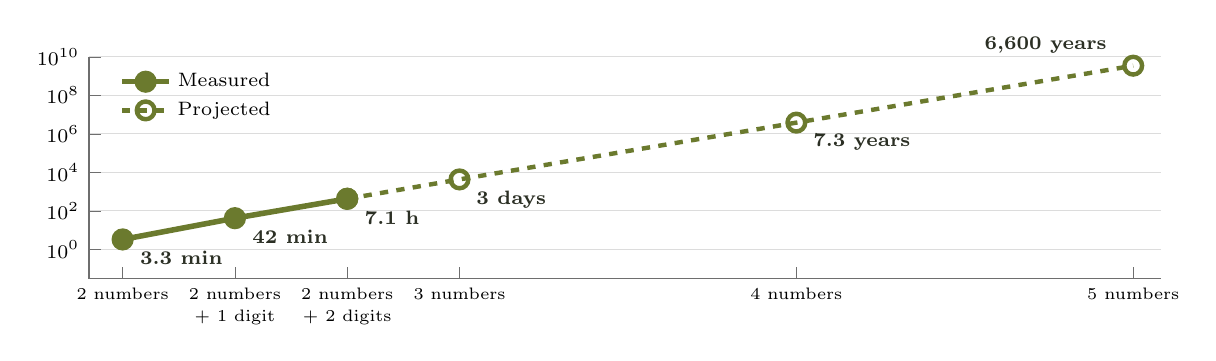
\begin{tikzpicture}
    \begin{axis}[
        width=15.2cm, height=4.4cm, clip=false,
        ymode=log, log basis y=10,
        ymin=0.03, ymax=1e10,
        ytick={1,1e2,1e4,1e6,1e8,1e10},
        yticklabels={$10^0$,$10^2$,$10^4$,$10^6$,$10^8$,$10^{10}$},
        xmin=-0.3, xmax=9.25,
        xtick={0,1,2,3,6,9},
        xticklabels={2 numbers,{2 numbers\\+ 1 digit},{2 numbers\\+ 2 digits},3 numbers,4 numbers,5 numbers},
        xticklabel style={font=\fontsize{6.5}{8}\selectfont,align=center,anchor=north,inner sep=3pt},
        yticklabel style={font=\scriptsize},
        ymajorgrids, grid style={gold!35},
        axis line style={muted}, tick style={muted},
        axis x line*=bottom, axis y line*=left,
        legend style={at={(0.02,0.98)},anchor=north west,draw=none,fill=none,font=\scriptsize},
        nodes near coords, point meta=explicit symbolic,
        every node near coord/.append style={font=\scriptsize\bfseries,color=navy,anchor=north west,xshift=2pt},
      ]
      \addplot[accent,line width=2pt,mark=*,mark size=3pt]
        coordinates {(0,3.3)[3.3 min] (1,42)[42 min] (2,426)[7.1 h]};
      \addlegendentry{Measured}
      \addplot[accent,line width=1.6pt,dashed,mark=o,mark size=3.2pt,mark options={solid,fill=white}]
        coordinates {(2,426)[] (3,4320)[3 days] (6,3.837e6)[7.3 years] (9,3.47e9)[]};
      \addlegendentry{Projected}
      \node[font=\scriptsize\bfseries,color=navy,anchor=south east,yshift=1pt] at (axis cs:8.85,3.47e9) {6,600 years};
    \end{axis}
  \end{tikzpicture}

  \vspace{0.1cm}
  {\color{muted}\tiny Enumeration time in minutes \textperiodcentered\ logarithmic scale \enspace|\enspace Projection assumes constant marginal cost per prefix, measured at digit 8.}
  \note{Target time: 45 seconds

The trie saves work, but the cost still grows exponentially with the length of the output: each extra digit multiplies the number of prefixes by about ten. Note that the vertical axis is logarithmic.

The filled points are measurements on one L40S GPU: about 3.3 minutes for two numbers, 42 minutes with one extra digit, and 7.1 hours with two extra digits.

The hollow points are projections. They assume each new prefix costs the same as we measured at the eighth digit. On that basis, three numbers would take about three days, four numbers about 7.3 years, and five numbers about 6,600 years. These are estimates, not experiments we ran.

Caching the states of every node would make each pass cheaper, but it would only shift this curve down; it would not change its slope. This is why we switch to Monte Carlo for longer outputs.}
\end{frame}

% =====================================================================
% 5. Monte Carlo
% =====================================================================
\setkicker{Method 2 \textbar\ Sample instead of enumerate}
\begin{frame}{Monte Carlo estimation using logits}
  \vspace{0.6cm}
  \centering
  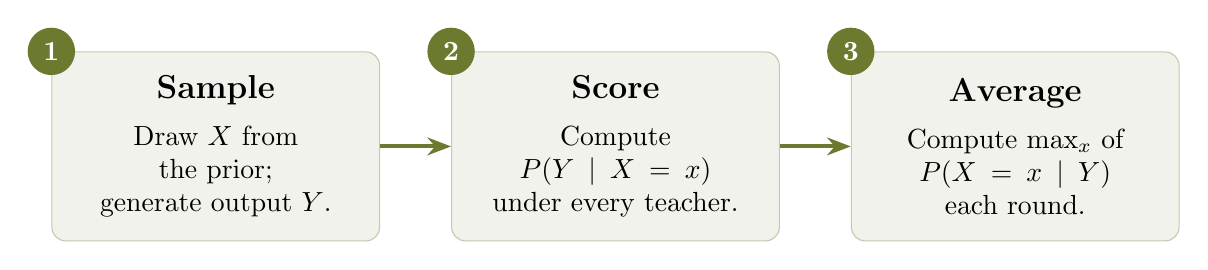
\begin{tikzpicture}[node distance=0.9cm,
      stepbox/.style={card,minimum width=3.9cm,minimum height=2.4cm,text width=3.6cm},
      num/.style={circle,fill=accent,text=white,font=\bfseries,inner sep=3pt},
      arr/.style={-{Stealth[length=3mm]},line width=1.4pt,color=accent}]
    \node[stepbox] (a) {{\large\bfseries Sample}\\[5pt] Draw $X$ from the prior;\\ generate output $Y$.};
    \node[stepbox,right=of a] (b) {{\large\bfseries Score}\\[5pt] Compute $P(Y \mid X = x)$\\ under every teacher.};
    \node[stepbox,right=of b] (c) {{\large\bfseries Average}\\[5pt] Compute $\max_x$ of\\ $P(X = x \mid Y)$ each round.};
    \node[num] at (a.north west) {1};
    \node[num] at (b.north west) {2};
    \node[num] at (c.north west) {3};
    \draw[arr] (a) -- (b);
    \draw[arr] (b) -- (c);
  \end{tikzpicture}

  \vspace{0.7cm}
  \takeaway{$V_1$ estimate = average of the largest posterior probability}

  \vspace{0.25cm}
  {\small Generate from the prior mixture and score with the same sampling rules.}
  \note{Target time: 40 seconds

Monte Carlo replaces enumeration with sampling from the channel marginal. First, draw a teacher condition from the prior. Then generate a sequence under that teacher. Score the same sequence under every possible teacher to calculate the posterior over secrets. Finally, average the largest posterior probability across sampled sequences. This is an unbiased estimator when we have the actual channel likelihoods. Generation and scoring must match, including masks and stopping rules. The filtered Gemma calculation additionally estimates acceptance probabilities and is therefore a plug-in estimate.}
\end{frame}

% =====================================================================
% 6. Validation
% =====================================================================
\setkicker{Validation \textperiodcentered\ Synthetic teachers}
\begin{frame}{Monte Carlo agrees with exact values}
  \vspace{0.6cm}
  \centering
  \renewcommand{\arraystretch}{1.35}
  {\small\setlength{\tabcolsep}{5pt}\begin{tabular}{ccccccc}
    \toprule
    \textbf{Length} & \textbf{Outputs} & \textbf{Exact $V_1$} & \textbf{MC estimate} & \textbf{95\% interval} & \textbf{Exact $\mathcal{L}^\times_1$} & \textbf{MC $\mathcal{L}^\times_1$} \\
    \midrule
    1 & 4   & 0.6000 & 0.5987 & [0.5972, 0.6003] & 1.800 & 1.796 \\
    2 & 16  & 0.6400 & 0.6412 & [0.6386, 0.6439] & 1.920 & 1.924 \\
    4 & 256 & 0.7624 & 0.7638 & [0.7612, 0.7664] & 2.287 & 2.291 \\
    \bottomrule
  \end{tabular}}

  \vspace{0.3cm}
  {\color{muted}\small Three secrets \textperiodcentered\ uniform prior \textperiodcentered\ 20,000 rounds \textperiodcentered\ $\mathcal{L}^\times_1=V_1(\pi,C)/V_1(\pi)$, with $V_1(\pi)=1/3$}

  \vfill
  \takeaway{Every exact value falls within its Monte Carlo 95\% interval.}
  \vspace{0.2cm}
  \note{Target time: 40 seconds

We first validate the estimator on a fully known synthetic channel with three teachers and four possible symbols. For each teacher, one symbol has probability 0.55 and the others have probability 0.15. With 20 thousand Monte Carlo rounds, all three exact values fall inside their corresponding 95 percent intervals. We also compare teacher-forced likelihoods with generation-time likelihoods for Qwen 0.5B and find a maximum reported difference within five times ten to the minus five. The intervals here measure Monte Carlo variability, not variation across training seeds.}
\end{frame}

% =====================================================================
% 7. Results Qwen 0.5B
% =====================================================================
\setkicker{Results \textperiodcentered\ Qwen2.5-0.5B-Instruct}
\begin{frame}{More observed lists reveal more information}
  \vspace{0.1cm}
  \centering
  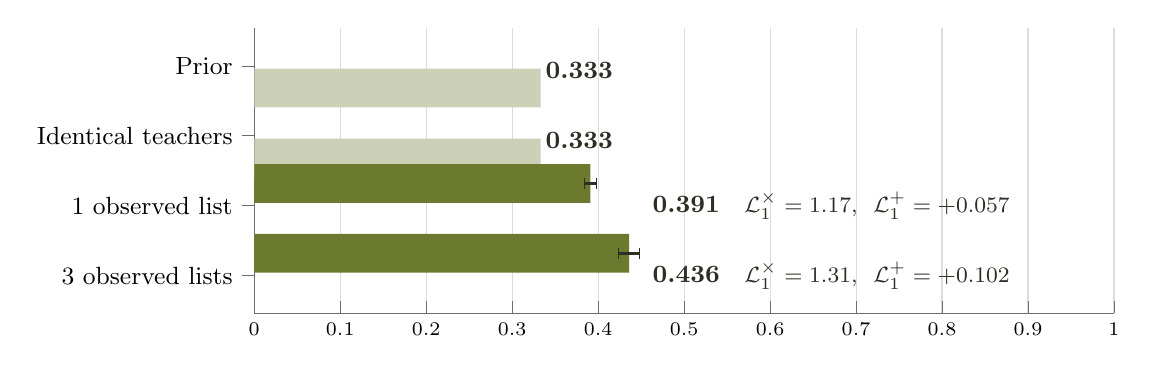
\begin{tikzpicture}
    \begin{axis}[
        xbar, width=12.5cm, height=5.2cm,
        xmin=0, xmax=1, bar width=14pt,
        y dir=reverse,
        ytick={0,1,2,3},
        yticklabels={Prior,Identical teachers,1 observed list,3 observed lists},
        yticklabel style={font=\small},
        xticklabel style={font=\scriptsize},
        xmajorgrids, grid style={gold!35},
        axis line style={muted}, tick style={muted},
        axis x line*=bottom, axis y line*=left,
        enlarge y limits=0.18,
        nodes near coords, point meta=explicit symbolic,
        every node near coord/.append style={font=\small\bfseries,color=navy,xshift=14pt},
      ]
      \addplot[fill=accent!35,draw=none] coordinates {(0.333,0)[0.333] (0.333,1)[0.333]};
      \addplot[fill=accent,draw=none,
               error bars/.cd, x dir=both, x explicit, error bar style={line width=1pt,navy}]
        coordinates {(0.391,2) +- (0.007,0)  (0.436,3) +- (0.012,0)};
      \node[font=\small\bfseries,color=navy,anchor=west] at (axis cs:0.452,2) {0.391 \enspace{\mdseries\footnotesize $\mathcal{L}^\times_1=1.17$, \ $\mathcal{L}^+_1=+0.057$}};
      \node[font=\small\bfseries,color=navy,anchor=west] at (axis cs:0.452,3) {0.436 \enspace{\mdseries\footnotesize $\mathcal{L}^\times_1=1.31$, \ $\mathcal{L}^+_1=+0.102$}};
    \end{axis}
  \end{tikzpicture}

  {\color{muted}\scriptsize Bar scale: 0 to 1; error bars: Monte Carlo 95\% intervals}

  \vspace{0.25cm}
  \takeaway{Three lists raise guessing success from 33.3\% to 43.6\% ($\mathcal{L}^\times_1=1.31$).}
  \note{Target time: 40 seconds

For Qwen 0.5B, the three teacher conditions favor owl, cat and dog through system prompting. One list asks for ten more numbers after the same fixed prefix, with generation limited to 40 tokens. Each trial with three lists uses the same teacher for all three independent generations. The prior success probability is one third. One list raises it to 0.391, and three lists to 0.436. The identical-teacher control stays at one third. These are modest average gains; the result does not imply that every individual list produces a posterior close to uniform.}
\end{frame}

% =====================================================================
% 8. Gemma
% =====================================================================
\setkicker{Leakage and behavioral transfer \textperiodcentered\ Dog preference}
\begin{frame}{Gemma: prompting versus fine-tuning}
  \vspace{0.15cm}
  \centering
  \renewcommand{\arraystretch}{1.35}
  {\small\setlength{\tabcolsep}{4pt}\begin{tabular}{lcccccc}
    \toprule
    \textbf{Induction} & \textbf{Raw $V_1$ ($\mathcal{L}^\times_1$)} & \textbf{Filtered $V_1$ ($\mathcal{L}^\times_1$)} & \textbf{Teacher} & \textbf{Student} & \textbf{Control} & \textbf{Effect (pp)} \\
    \midrule
    Prompt      & 0.9284 (1.86) & 0.9045 (1.81) & 57.2\% & 8.47\%  & 5.27\% & {\color{accent}\bfseries +3.20} \\
    Fine-tuning & 0.9971 (1.99) & 0.9999 (2.00) & 100\%  & 16.93\% & 6.67\% & {\color{accent}\bfseries +10.27} \\
    \bottomrule
  \end{tabular}}

  \vspace{0.25cm}
  {\color{muted}\scriptsize
  Same base model and target preference; two ways to induce the teacher trait.\\
  Dog-preference rates (\%). Effect = student minus control (percentage points).\\
  QIF: 1,000 samples, one list; $\mathcal{L}^\times_1=V_1/0.5$, at most 2 for a binary secret \enspace|\enspace Student and control: means over three seeds}

  \vspace{0.2cm}
  \takeaway{High distinguishability alone does not establish strong preference transfer.}

  \vspace{0.15cm}
  {\small Filtered $V_1$ concerns accepted token paths; decoded text may reveal less information.}
  \note{Target time: 55 seconds

We next compare two Gemma 2 9B teachers. One receives the dog preference as an instruction prepended to the user message. The other has a fine-tuned adapter. Each is compared with the unmodified base model, so prior vulnerability is one half. We estimate QIF with one thousand samples and one observed list. Students train on ten thousand accepted numeric continuations; behavioral results average three training seeds with five hundred evaluation responses per model. Both channels are highly distinguishable. Fine-tuning yields higher vulnerability and a larger average increase in dog preference. But prompting already has high vulnerability while producing only a small average effect, with a negative effect in one seed. Filtering conditions on acceptance, so higher filtered vulnerability does not violate data processing. These two conditions do not establish predictive power.}
\end{frame}

\end{document}